\section{System-level modeling}
\label{sec:esd-modeling}

% Simulations are a key tool
Among all investigations and analysis methods, simulations are extremely important for understanding the impact of \gls{esd}s on integrated circuits.
Physical access to signals and nets is extremely difficult in the actual chip, while in simulation it is straightforward.
Like testing and measurement methods, simulations are another valuable tool for \gls{esd} analysis.

% But require a lot of preliminary effort
However, \gls{esd} simulations are far from trivial
For operating ESD, need electrical device models that work in normal operating conditions and in electrostatic domain of fast transients, highly non-linear and rapidly changing signals.
To build trust on the simulation results, models must be validated against measurement data, and in many different test conditions.

% Hierarchical level
Electronic systems are by nature hierarchical systems.
Large scale devices like test generators interact with small scale devices like integrated circuits, themselves composed of transistors and other integrated devices.
For \gls{esd} simulations, it is not always obvious a what scale the modelling effort must be made.
There is always a compromise between the model accuracy, modelling time and effort, and simulation speed.

% Which level is targeted here
In this chapter, a methodology for building electrical models of systems and electrical setups is proposed.
Some concepts also apply at the board level.

% Main concept
A modular approach is adopted.
At the system level, \gls{esd} generator and lab equipments must modeled.
Electronic systems and test setups are very often composed of a limited set of standard and common devices.
Equipments are made for example of DC sources, discrete passive devices, relays.
Equipments are connected together with the use of wires, twisted wire pairs, coaxial cables, etc.
The goal is to build a library of those discrete devices.
Each model of the library is qualified independently with measurements.
At the system level, physical access to most electrical nets of a circuit is easy, simplifying measurement and verification of the models.
Later on, the architecture or the electrical circuit of a system serves as a blueprint for modelling it.
It is assembled by connecting models from the library together.

% Limits in voltage/time
Models described hereafter target two kinds of simulation
DC or normal operation transient simulations
\gls{esd} simulations, with accuracy near the nanosecond and voltage or current levels well above normal operating conditions.
At such short timespan, and with the usual dimensions of \gls{esd} test equipment and \gls{pcb}, electrical propagation effects are no longer negligible.
% TODO Non-linear behavior ?


\subsection{Transmission line}

%TODO: Emphasize that a good line model is essential given how often the TLP is used for analysis in the ESD field

% Cables and delays identified as important for esd sims - because of similar order of magnitude
Among all devices used in \gls{esd} test setups, cables were found critical for modelling and simulation.
In a standard 50\textOmega{} coaxial cable, it is common to find propagation delays in the range of 5 ns/m.
Cable lengths in laboratories usually measure between tens of centimers to one or two meters.
Thus, it is common to find delays in the order of 1 ns to 10 ns.
On the other hand, electrostatic discharges last a few hundred 100 ns.
Both values are near the same order of magnitude, which justifies why cables and delays in general should be taken into account in fast transient simulations.

% Also consider not just the delay but the oscillations
Beyond simply adding a delay and offsetting a signal in time, delays can also be involved in ringing oscillations if the circuit contains impedance mismatches.
In this situation, delay belows the nanosecond can have a strong impact on waveforms.
Delays of this order of magnitude are commonly found in \gls{pcb} metal tracks.
Beyond coaxial cables and \gls{pcb} traces, any element that generates a significant delay should be modelled.

% How to model delays ? with lossless TL
Cables, metal traces and wires in different configurations were all found to behave as transmission lines.
More specifically, for frequencies below a GHz, most cables and tracks can be modelled as lossless transmission lines.

% What is a transmission line ?
A transmission line is an electrical propagation media.
Physically, it can be seen as a succession of infinitely small unit elements.
Each element is modeled by an inductance, a capacitance and sometimes a leakage resistance or conductance.
A transmission line can also be defined by a characteristic impedance Z\textsubscript{c} and a propagation delay \textDelta{}t.
A \gls{Zc} is the ratio of the amplitudes of voltage and current of a single wave propagating along the line.
Equation \ref{eq:characteristic-impedance} relates the characteristic impedance to the unit line inductance \textdelta{}L and capacitance \textdelta{}C.

\begin{equation}
Z_{c} = \sqrt{\frac{\delta L}{\delta C}}
\label{eq:characteristic-impedance}
\end{equation}

% Lossless is an approximation
In practice, truly lossless cables do not exist but below a few GHz the lossless approximation is valid.
A lossless line exhibits a purely real characteristic impedance.

\subsubsection{Distributed model}
% Distributed model
The most popular line model is based on a distributed capacitance and inductance.
The model is a series of unit LC elements as illustrated in Fig. \ref{fig:dis-line-model}.
The value for this unit element can be computed from the characteristic impedance \gls{Zc} with Eq. \ref{eq:characteristic-impedance}.

\begin{figure}[!h]
  \centering
  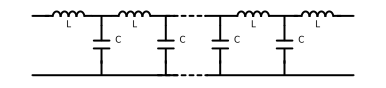
\includegraphics[width=0.7\textwidth]{src/2/figures/lc_ladder.pdf}
  \caption{Electrical distributed LC ladder model of a lossless transmission line}
  \label{fig:dis-line-model}
\end{figure}

\begin{equation}
\delta t = \sqrt{\delta L.\delta C}
\label{eq:unit-delay}
\end{equation}

% A string of unit elements form the total model
Each element induces a propagation delay \textdelta{}t, whose values can be computed from the unit inductance and capacitance with Eq. \ref{eq:unit-delay}.
In a string of connected unit elements, the individual delays add up.
With enough elements, the delay and behavior of the complete cable is reproduced.

% Tradeoff between amount of elements and
During modelling, it is tempting to take large values for \textdelta{}L and \textdelta{}C, to get a large unit delay.
Doing so reduces the amount of unit elements, and speeds up the simulation.
However, there is a tradoff between the delay of the unit element and the accuracy of the simulation.
A smaller unit delay increases accuracy of the model at large frequencies, but more elements are required for the total cable, resulting in longer simulation times.
On the other hand, a larger unit delay reduces the bandwidth of the model, which may be unsuitable for accuracy, even if simulation times are improved.

% How to calculate the unit values ?
%TODO
Resolving equation system \ref{eq:characteristic-impedance} and \ref{eq:unit-delay}.

\begin{equation}
L = \frac{Z_{C}.\delta t }{N}}
\label{eq:unit-inductance}
\end{equation}

\begin{equation}
C = \frac{\delta t}{N.Z_{C}}}
\label{eq:unit-capacitance}
\end{equation}

% Perks and disavantages
The distributed model supports easily lossy transmission lines by adding a unit resistance or conductance between signal and ground, or in series with the signal.
On the other hand, this model does not scale well as cables get longer.
To keep the same bandwidth with a longer cable, the only solution is to increase the element count, resulting in longer simulation time.
Also, this model will always be bandwidth limited, otherwise it would require an infinite amount of infinitely small elements.

\subsubsection{Behavioral model}

% Behavioral model
%TODO: Reference to article
A behavioral model is an excellent alternative to the distributed model.
It can describe efficiently and with great accuracy the behavior of most lossless transmission lines.
The model is constituted of two voltage-controlled voltage sources and two resistors (Fig. \ref{fig:beh-line-model}).
Compared to the distributed model, the behavioral model has by design an infinite bandwith, and is extremely fast to simulate.
It also is constant in complexity, because the simulation time is independant of the cable's delay or required bandwidth

\begin{figure}[!h]
  \centering
  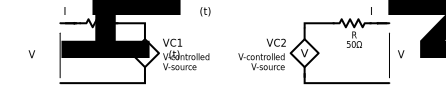
\includegraphics[width=\textwidth]{src/2/figures/behavioral_line_model.pdf}
  \caption{Electrical behavioral model of a lossless transmission line}
  \label{fig:beh-line-model}
\end{figure}

Equations \ref{eq:beh-line-1} and \ref{eq:beh-line-2} describe the behavior of the voltage-controlled voltage sources.

\begin{equation}
V_{C1}(t) = V_{2}(t - \Delta t) + Z_{C}.I_{2}(t - \Delta t)
\label{eq:beh-line-1}
\end{equation}

\begin{equation}
V_{C2}(t) = V_{1}(t - \Delta t) + Z_{C}.I_{1}(t - \Delta t)
\label{eq:beh-line-2}
\end{equation}

% Explain the equations
Z\textsubscript{C} is the characteristic impedance of the line and \textDelta{}t the propagation delay between both ports.
Overall, the equations describes a system where voltage and current at both ports are defined by the combination of a forward travelling wave and a backward travelling wave.
An example implementation in VHDL-AMS is provided in Listing \ref{lst:tline}.

\begin{code}
\inputminted[frame=single]{VHDL}{src/2/snippets/tline.vhdl}
\label{lst:tline}
\caption{Transmission line behavioral VHDL-AMS model}
\end{code}


\subsubsection{Comparison}

% Compare both models to know which one is preferrable
Simulations are ran to compare both models.
The setup is given in Fig. \ref{fig:lines-testbench} and consists in injecting a rectangular pulse with a risetime of 1 ps into a load through the modelled transmission line.
Different load values are employed to observe the performance and accuracy of each model.
The transmission line to model has been chosen to a delay of 100ns and a characteristic impedance of 50 \textOmega.
Both values correspond to the cable usually employed in a transmission line pulsing generator and are thus very realistic.

%TODO: Simulation with 10

\begin{figure}[!h]
  \centering
  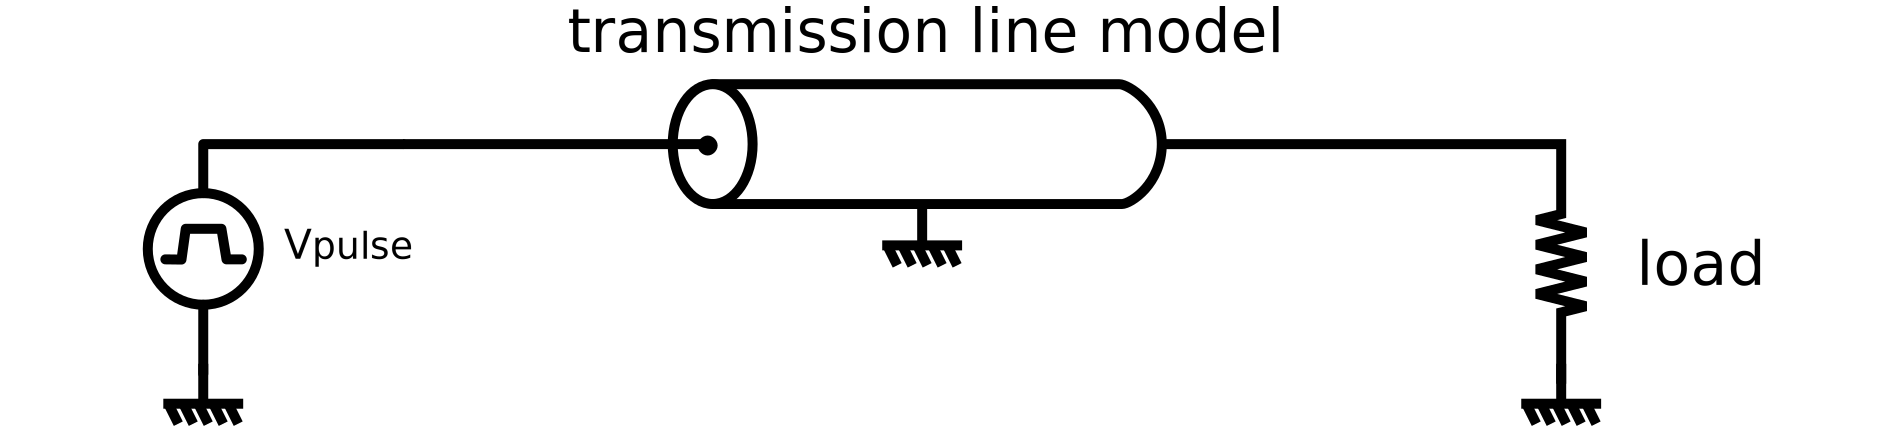
\includegraphics[width=0.8\textwidth]{src/2/figures/tline_validation_setup.pdf}
  \caption{Line model validation testbench}
  \label{fig:lines-testbench}
\end{figure}

Overall, the behavioral model outperforms the distributed model for representing a perfect transmission line.
It reproduces exactly the 1ps risetime on the load in all configurations (Fig. \ref{fig:lines-simulations}).
The distributed model is either not as accurate or much slower to simulate.

\begin{table}[!h]
\centering
\begin{tabular}{@{}lllll@{}}
\toprule
amount N         &  10           & 100        &  1000      &   10000    \\ \midrule
simulation time  &  15 ms        & 170 ms     &  7.5 s     &   135 s    \\
increase ratio   &  -            & x10        &  x44       &   x18      \\
\bottomrule
\end{tabular}
\caption{Impact of the amount of unit elements on the simulation times}
\label{tab:tline-impact-simulation-time}
\end{table}

For good accuracy, individual delay must be 2 or 10 times smaller than the shortest rise time.
Also, simulators with variable timestep have trouble reproducing appropriately oscillating events with good accuracy for the period.
So with the LC line, the waveform is mostly noise or assimilated to it.
Oscillations also force the simulators to fall back to the smallest timestep, considerably increasing simulation time and data output size.

For a 100ns TLP with 100ps risetime, individual delay is 10ps.
N = 100e- / 10e-12 = 1e4 elements which is rather huge and will increase simulation time.

\begin{figure}[!h]
  \centering
  \includegraphics[width=0.3\textwidth]{src/2/figures/tline_models_comparison.pdf}
  \caption{Models comparison in simulation}
  \label{fig:lines-simulations}
\end{figure}

Even 10000 elements are not enough for obtaining a clean risetime.


In conclusion, the behavioral model should be preferred wherever possible.
The distributed model should be used in cases where losses must be taken into account, which is rather rare in practice.

\subsection{Passive devices}

% Limitations of passive devices
Properties of passive devices such as capacitors, resistors and inductors change in particular electrical conditions \cite{capa-esd-cz}.
For large transient amplitudes above nominal range and high-frequencies, their nominal values easily vary by an order of magnitude.
At frequencies above a few MHz, the parasitic devices play an important role and make the device ineffective at some point.
For instance, capacitors exhibit an inductive behavior for sufficiently large frequencies.

% In what frequency range are ESD active, and are those limitations in effect
Electrostatic discharges have been characterized in the frequency domain in \cite{fft-esd}.
It concerns air discharges and non-shielded discharges that radiate heavily.
The spectrum of the IEC 61000-4-2 standard \cite{iec61000-4-2} was recorded.
It is shown that the majority of the frequency content is below 1GHz, with important magnitudes until tens of MHz.
Like indicated previously, this is the frequency range where parasitic behavior is important.
Therefore for \gls{esd} simulations, passive devices require models that take those parasitic devices into account.

% Not all device need parasitic device modelling
In practice, it was found that only some passive devices in a system have a notable impact on the waveform at high-frequencies.
For others, using a regular electrical model is sufficient.
Decoupling capacitors were noticed to require parasitic device modelling.
Since they are connected between a voltage reference (supply voltage) and a reference (ground), they have a strong impact on the disturbance waveforms that an \gls{ic} pin is exposed to.
Passive device models working at frequencies below 1GHz are given in Fig. \ref{fig:rlc-esd-models} for inductors, resistors and capacitors.

\begin{figure}[!h]
  \centering
  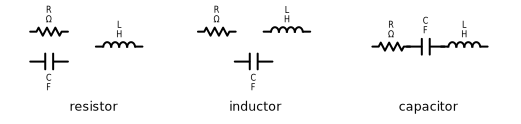
\includegraphics[width=\textwidth]{src/1/figures/rlc_models.pdf}
  \caption{High-frequency (< 1GHz) models for resistor, capacitor and inductor}
  \label{fig:rlc-esd-models}
\end{figure}

% How to tune those models
Those models are easily parameterized.
Values can be extracted with an impedance meter capable of measuring impedances to at least 100 MHz.
Fig. \ref{fig:frequency-response-capa} displays the magnitude and phase versus frequency of a 6.8 nF \gls{smd} capacitor.
The capacitor exhibits a perfect behavior up to 45MHz.
The slope of the curve below 45 MHz is directly related to the capacitor value (see Equation \ref{eq:capacitor-impedance}).
Below 45 MHz, the phase has a value of $-90$ degrees, corresponding to the theory.

%TODO: Check this equation
\begin{equation}
\delta M/ \delta f = C. \omega = 2.\omega .C.f
\label{eq:capacitor-impedance}
\end{equation}

% What are the parasitic devices in this curve
At the resonant frequency, the capacitor is equivalent to a non-ideal short-circuit, basically a low-value resistor.
This resistor, also called \gls{esr}, is both a parasitic device and the series resistance in the high-frequency model presented earlier.
Beyond 45 MHz, the capacitor behaves as an inductor.
The phase shift is the one of an inductor at $+90$ degrees.
This second slope is determined by the parasitic inductor value (see equation \ref{eq:inductor-impedance}).
In conclusion, the values for parasitic inductor and resistor can be computed very easily from a measurement.

\begin{equation}
\delta M/ \delta f =  -L.\omega = -2.\omega .L.f
\label{eq:inductor-impedance}
\end{equation}

\begin{figure}[!h]
  \centering
  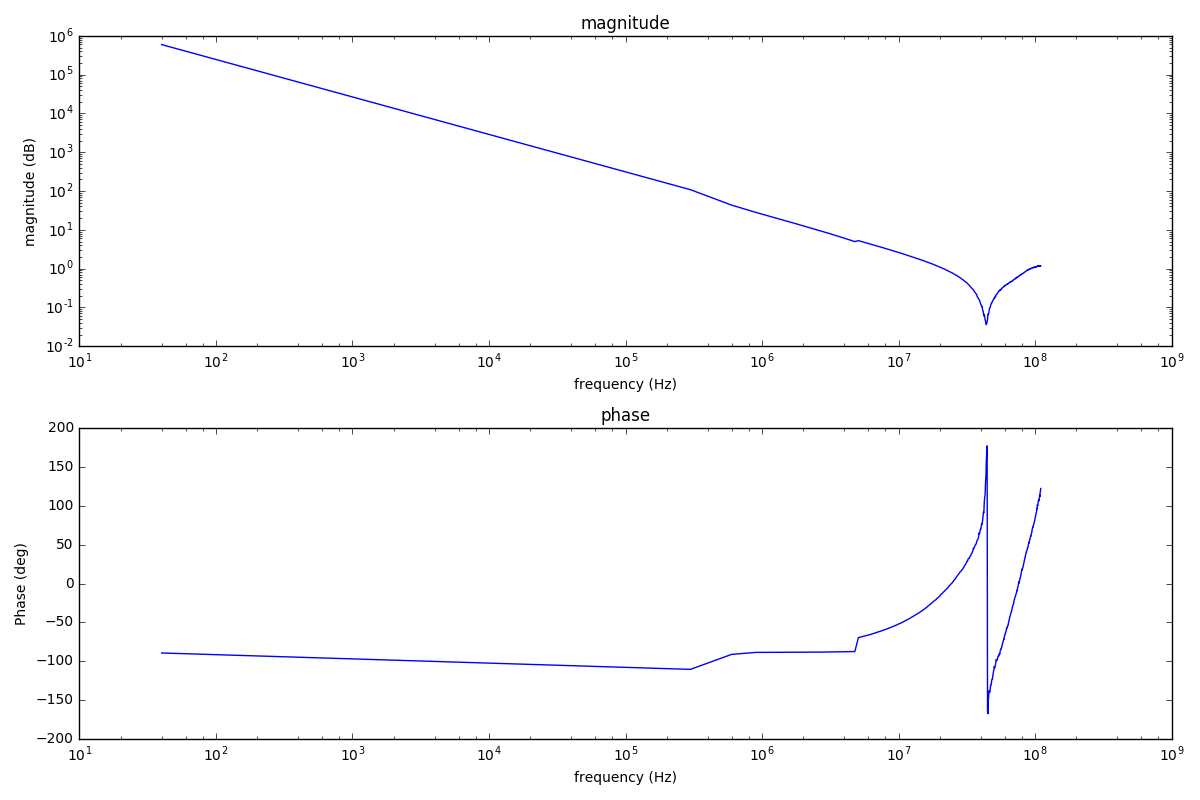
\includegraphics[width=0.3\textwidth]{src/1/figures/capa_hf_response.png}
  \caption{Frequency response of a 6.8nF capacitor}
  \label{fig:frequency-response-capa}
\end{figure}

% Impact of dimensions on parasitic values
%TODO: Quote fabien ? Or find reference
In the case of capacitors, for a given package, first observations tend to show few variations for the parasitic inductance, even with capacitors of different values and sizes.
The parasitic inductance seems mostly related to the kind of package, and measured values are between 1nH and 5nH.
This observation tends to indicate that there is no need to characterize every single passive device.
Instead, a global parasitic model per package should suffice.

% Non-linear high power behavior
%TODO: Quote fabien
%TODO: Find articles that show non-linear behavior
So far, only the frequency-related behavior was detailed.
For high power and amplitudes, most passive devices also suffer of nominal ratings variations.
\gls{mlcc} are concerned about this phenomenon \cite{capa-esd-cz}, where the capacitance decreases at high voltages.
On the contrary, capacitors built with the X7R technology are much most resilient in high regime conditions and exhibit little variations.

% Conclusion
%TODO

\subsection{Other devices}

%TODO: A etoffer

% Diodes
Diodes and \gls{tvs} are frequently studied devices in the \gls{esd} field \cite{modelling-diode-esd, esd-diode-compact-model, tvs-modeling}.
Multiple modelling methods exist, such as behavioral and compact models.
Most studies target silicon-level devices, but a few also interested in board-level active device modelling.

% Common mode choke
Common mode choke are frequently encountered in electronic systems to protect inputs and supplies in particular \cite{cmc-for-emc-protection, cmc-esd, alternative-cmc-emi-noise}.
Unlike regular RC-network filtering, chokes isolate from common mode disturbances where both signal and ground reference voltages shift.
Chokes are frequently used for reducing emmission in \gls{emc} tests, and increasing immunity of a system to conducted disturbances.


\subsection{Propagation phenomena}

%TODO
Sometimes important to take into account for the modelling and assembling of models

Propagation and reflection are the two main phenomena occurring at the nanosecond timescale that are ignored in standard time-domain electrical simulations.

Propagation is a phenomenon that always occurs but is negligible over a few tens microseconds.
Below that timescale it must be taken into account because it has a major impact on the waveforms.
This is due to the fact that observation times are in the same range than electrical wave propagation times.

Reflection happens when an electrical wave propagates and reaches a point where two propagation media are mismatched (two coaxial cables of different characteristic impedance for example).

These two effects and in combination can impact waveform in some specific scenario

% Measurement artifact
Spike visible on measurements but is just an artifact
Caused by a delay between an intended measurement point and where the measurement is actually performed
Delay because of a cable for instance
Setup given in Fig \ref{fig:setup-measurement-spike}

\begin{figure}[!h]
  \centering
  \includegraphics[width=0.3\textwidth]{src/1/figures/setup_measurement_spike.pdf}
  \caption{Typical setup causing a measurement artifact}
  \label{fig:setup-measurement-spike}
\end{figure}

The process that generates this measurement glitch starts with the injection of a fast rectangular pulse.
The pulse propagates towards point A (step 1).

\begin{figure}[!h]
  \centering
  \includegraphics[width=0.3\textwidth]{src/1/figures/spike_generation_1.pdf}
  \caption{Spike generation - step 1}
  \label{fig:spike-step-1}
\end{figure}

At the moment it reaches A, the capacitor load is not immediately visible.
It is “hidden” from point A by the short delay.
Thus, the voltage rises, depending at this point only on the characteristic impedances of the cables.
A part of the pulse propagates towards the load and a part toward Vout (depending on the impedance ratio) (step 2).

\begin{figure}[!h]
  \centering
  \includegraphics[width=0.3\textwidth]{src/1/figures/spike_generation_2.pdf}
  \caption{Spike generation - step 2}
  \label{fig:spike-step-2}
\end{figure}

The impulse reaches then the load (step 3), and propagates back toward A, settling the voltage at A to
V – (V – Vload) = Vload (forward travelling wave minus reflected wave from load) (step 3).
The capacitor is supposed to be charging at constant current, voltage rises following a linear curve.

\begin{figure}[!h]
  \centering
  \includegraphics[width=0.3\textwidth]{src/1/figures/spike_generation_3.pdf}
  \caption{Spike generation - step 3}
  \label{fig:spike-step-3}
\end{figure}

Now the voltage at point A is defined by the load.
However before that, the voltage rose and generated a peak that will hit Vout after a delay.
This peak preceding the capacitor charge is detailed on figure \ref{fig:spike-step-4}.
The amplitude is exaggerated for illustration purposes

\begin{figure}[!h]
  \centering
  \includegraphics[width=0.3\textwidth]{src/1/figures/spike_generation_4.pdf}
  \caption{Spike generation - step 4}
  \label{fig:spike-step-4}
\end{figure}

In a more realistic situation, if the short delay is of the same order of magnitude than the pulse risetime, the generated peak will be a non-negligible fraction of the initial pulse amplitude.

\begin{figure}[!h]
  \centering
  \includegraphics[width=0.3\textwidth]{src/1/figures/spike_generation_5.pdf}
  \caption{Measured waveform}
  \label{fig:spike-step-4}
\end{figure}

% Unterminated cables
Because of propagation and reflection phenomena, elements that are normally ignored in standard simulations can no longer be neglected.
A perfect illustration of this point are cables connected to the circuit on one end, and left floating on the other end (or in high impedance)
In regular simulations, they can removed entirely.
With ESD simulations, they will induce oscillations and amplitude changes

\begin{figure}[!h]
  \centering
  \includegraphics[width=0.3\textwidth]{src/1/figures/setup_unconnected_cable.pdf}
  \caption{Typical setup causing oscillations}
  \label{fig:setup-unconnected-cable}
\end{figure}

%TODO: Rewrite completely
Transient current propagates toward the unconnected end
Reflects entirely at the high impedance termination
Comes back inside the circuit, absorbing a part of the initial current and supplying it later on.
The consequence is an undershoot followed by a delayed overshoot (fig. 15).
%TODO: Put a waveform ?

\gls{tlp} is a perfect example of an application exploiting an unterminated cable

% Feeding cables
%TODO: Talk about location of measurement point
Similarly, all cables on the propagation path (Fig. \ref{fig:setup-feeding-cable}) must not be neglected just because they are matched with the circuit.
The delay they introduce impacts greatly the waveforms.
TLP generators always require a cable to connect the load under test to the generator.
This connection cable plays a role in the final waveform.
In simulation, if omitted, the waveform is very rectangular and clean (Fig. \ref{fig:comparison-feeding-cable}).
When the cable is added, the presence of reflections with this delay changes quite a lot the waveform that now has an initial step between 00 and XX ns, with an amplitude corresponding to the TLP charging voltage and not the circuit operating point
XX ns corresponds exactly to (twice ?) the delay of the feeding coaxial cable.

\begin{figure}[!h]
  \centering
  \includegraphics[width=0.3\textwidth]{src/1/figures/setup_feeding_cable.pdf}
  \caption{Minimal TLP generator with feeding cable and a mismatched load}
  \label{fig:setup-feeding-cable}
\end{figure}

\begin{figure}[!h]
  \centering
  \includegraphics[width=0.3\textwidth]{src/1/figures/comparison_feeding_cable.png}
  \caption{Simulated waveform with and without feeding cable}
  \label{fig:comparison-feeding-cable}
\end{figure}

% Conclusion
%TODO: Detail
Beyond these particular examples, the idea is to be cautious about even short delays when assembling models from the library.
